\section{Сетевой анализ рынка}
Прежде чем приступить к изучению мер неопределённости, рассмотрим вопрос построения рыночных сетевых структур на основе разных мер близости. Предположим, что мы хотим построить граф, основываясь на наблюдениях за $N$ акциями в течении $n$ дней. Данные представляют собой цены акций в момент закрытия торгов в каждый из дней. В первую очередь, имеющиеся данные мы преобразуем в данные о ежедневной доходности акций. Доходность акции $k$ в день $t$ рассчитывается как	
\begin{equation}
	R_k(t)=\ln\frac{P_k(t)}{P_k(t-1)}
\end{equation}
где $P_k(t)$ -  цена акции $k$ в день $t$. 

Предположим, что для некоторого фиксированного $k$ и $t=1,...,n$ $R_k(t)$ - независимые одинаково распределённые случайные величины и имеют такое же распределение, что и случайная величина $R_k, k=1..N$. Можно также предположить, что случайные величины $R_1, ... ,R_N$ имеют совместное нормальное распределение. В этом случае выборочная матрица корреляции $||r_{i j}||$ будет содеражать большую часть доступной информации о зависимости этих случайных величин\cite{anderson}. Каждый элемент такой матрицы вычисляется как 

\begin{equation}
	r_{i j} = \frac{ \sum_{t=1}^{n} (R_i(t) - \overline{R_i})(R_j(t) - \overline{R_j})  }{ \sqrt{ \sum_{t=1}^{n} (R_i(t) - \overline{R_i})^2 }\sqrt{ \sum_{t=1}^{n} (R_j(t) - \overline{R_j})^2 } }
\end{equation}

где $\overline{R_i} =  \frac{1}{n}\sum_{t=1}^{n} R_i(t)$ - выборочное среднее $R_i$. Такая матрица часто используется в качестве меры близости в сетевой структуре, отражающей структуру фондового рынка.

Однако, если появляются какие-то отклонения совместного распределения случайных величин от нормального, матрица $||r_{i j}||$ перестанет полностью характеризовать взаимосвязь между случайными величинами. Изучение этих отклонений и влияние их на статистическую неопределённость сетевых структур являются одной из целей данной работы. 

Чтобы смоделировать подобные отклонения, предположим, что доходности имеют смешанное распределение: часть наблюдений распределена согласно нормальному закону, а остальные имеют распределение Стьюдента. Введём параметр $r \in [0,1]$, который будет отвечать за то, какая доля наблюдений иметь распределение Стьюдента.

Один из общих подходов построения многомерного распределения Стьюдента (или t-распределения) размерности $p$, описанный в \cite{t-distrib}, состоит в следующем. Пусть $Y$ и $u$ - независимые и распределеные как $Y \sim N(0, \Sigma)$ и $u\sim\chi_\nu^2$, где $\Sigma$ - квадратная матрица размерностью $p \times p$. Пусть $T$ такая что
\begin{equation}
  \frac{Y}{\sqrt{u/\nu}} = T - \mu 
  \label{eq:student}
\end{equation}

Тогда $T$ иммет многомерное распределение Стьюдента с параметрами $\Sigma, \mu, \nu$:  $T \sim t_\nu(\mu, \Sigma)$. Заметим, что матрица $\Sigma$ не является матрицей ковариации. Матрица ковариации определяется как $\frac{\nu}{\nu-2}\Sigma$ для $\nu > 2$. В этой работе будем использовать параметр $\nu = 3$.
	
	
В работе \cite{signs} была представлена мера близости, которую можно использовать  в условиях подобных отклонений. Эта мера основана на вероятности совпадений знаков доходностей. Она позволяет описать совместное поведение случайных величин $R_1, ..., R_N$ даже если совместное распределение случаных величин неизвестно. Она определяется как

\begin{equation}
	p_{i j} = P(R_i \geq E(R_i), R_j \geq E(R_j) \cup R_i < E(R_i), R_j < E(R_j))
\end{equation}

В этой работе мы будем использовать схожую меру - выборочная вероятность совпадения знаков:
\begin{equation}
	\gamma_{i j} = \frac{1}{n}\sum_{t=1}^{n}I[R_i(t)R_j(t)]
\end{equation}
где 
\begin{equation*}
  I[x] =
    \begin{cases}
      1, & \text{если $y \geq 0 $}\\
      0, & \text{если $y < 0 $}\\
    \end{cases}       
\end{equation*}


Фондовый рынок можно представить как конечный полный взвешенный неориентированный граф без петель и кратных рёбер $G=(V,E)$, где $V={1,2,...,N}$  - множество вершин, соответствующее наименованиям акций, а $s_{i j}$ - вес ребра $(i,j) \in E$, отражающий значение некоторой меры близости соответствующих акций. Такой граф мы будем называть рыночной сетевой структурой. В этой работе будут рассмотрены структуры, основанные на двух мерах близости: выборочной корреляции Пирсона и выборочной вероятности совпадения знаков.  В зависимости от выбранной структуры, матрицей весов графа будет либо $||r_{i j}||$  для выборочной корреляции Пирсона, либо $||\gamma_{i j}||$  для выборочной вероятности совпадения знаков.


\subsection{Процедуры фильтрации}

Для извлечения наиболее ценной информации из сетевой структуры и упрощения дальнейшего анализа используются различные процедуры фильтрации, которые предполагают построение подграфа исходной сети. Мы будем рассматривать следующие процедуры:

\begin{enumerate}
	\item Построение максимального остовного дерева (maximum spanning tree)
	\item Построение рыночного графа (market graph)
	\item Построение максимальной клики на основе рыночного графа (maximum clique)
	\item Построение максимального независимого множества на основе рыночного графа (maximum independent set)
\end{enumerate}

Остовное дерево связанного графа представляет собой связанный подграф, содержащий все вершины исходного подграфа и не имеющий циклов.  Максимальное остовное дерево - это остовное дерево, имеющий максимальный вес, который вычисляется как сумма весов ребёр, входящих в остовное дерево. Мы рассматриваем именно максимальное остовное дерево, так как заинтересованы в том, чтобы найти наиболее тесно связанные между собой акции относительно показателей их доходностей. Использование этой процедуры было предложено в \cite{mst2}.

Позднее, в работе \cite{mg} был представлен и изучен рыночный граф (market graph), который получается из исходного путём удаления всех рёбер, веса которых меньше некоторого заданного значения порога $\theta$. В полученном графе можно найти максимальную клику и максимальное независимое множество, с помощью которых можно проанализировать структуру фондового рынка, а максимальное независимое множество можно рассматривать как основу для создания диверсифицированного портфеля акций. В неориентированном графе кликой называют подмножество вершин, которые порождают полный подграф исходного графа. Максимальная клика графа - это клика максимального размера, то есть включающая в себя максимально возможное число вершин. Независимое множество - понятие, обратное понятию клики. Это подмножество вершин графа, не имеющих общих рёбер. Максимальное независимое множество - это назависимое множество максимального размера.

При построении  рыночного графа, а также максимальной клики и максимального независимого множества на основе сети, веса в которой представляют собой выборочную вероятность совпадения знаков возможно установить связь между классической корреляцией Пирсона и корреляцией знаков\cite{signs}. Обе меры связаны соотношением

\begin{equation}
	\theta_\gamma = \frac{1}{2}\left(\frac{2}{\pi}\arcsin\theta_r +1\right)
	\label{eq:threshold}
\end{equation}

Таким образом, мы сможем сравнить статистическую неопределённость структур, построенных на основе разных мер близости. Выбрав порог $\theta_r$ для построения рыночного графа на основе корреляции Пирсона, мы можем расчитать порог $\theta_{\gamma}$ для рыночного графа на основе корреляции знаков. Меры неопределённости для полученных структур будут сравнимы дург с другом.



\subsection{Пример}

Рассмотрим пример построения сети на основе корреляции Пирсона для следующего набора акций NASDAQ: 

{ \small
\begin{enumerate}
  \item AAPL (Apple)
  \item AMZN (Amazon)
  \item CZR (Caesars Entertainment Corporation)
  \item GOOG (Alphabet Inc.)
  \item LBTYA (Liberty Global)
  \item NAVI (Navient)
  \item PEP (PepsiCo Inc.)
  \item PTLA (Portola Pharmaceuticals)
  \item SFM (Source Filmmaker)
  \item XOG (Extraction Oil \& Gas)
\end{enumerate}
}
В качестве меры близости будем использоват корреляцию Пирсона. Имея данные о ценах этих акций за 2018-2019, рассчитаем их доходности и составим матрицу выборочной корреляции Пирсона $ ||r_{ij}|| $. Матрица будет иметь вид:

{ \tiny
\kbordermatrix{\mbox{}&AAPL&AMZN&CZR&GOOG&LBTYA&NAVI&PEP&PTLA&SFM&XOG\\
AAPL&1.000&0.626&0.337&0.631&0.309&0.354&0.270&0.352&0.151&0.326\\
AMZN&0.626&1.000&0.451&0.702&0.334&0.337&0.181&0.341&0.152&0.279\\
CZR&0.337&0.451&1.000&0.422&0.278&0.358&0.143&0.276&0.086&0.232\\
GOOG&0.631&0.702&0.422&1.000&0.344&0.327&0.244&0.384&0.157&0.242\\
LBTYA&0.309&0.334&0.278&0.344&1.000&0.338&0.175&0.206&0.029&0.258\\
NAVI&0.354&0.337&0.358&0.327&0.338&1.000&0.156&0.276&0.189&0.310\\
PEP&0.270&0.181&0.143&0.244&0.175&0.156&1.000&0.115&0.042&0.075\\
PTLA&0.352&0.341&0.276&0.384&0.206&0.276&0.115&1.000&0.077&0.201\\
SFM&0.151&0.152&0.086&0.157&0.029&0.189&0.042&0.077&1.000&0.105\\
XOG&0.326&0.279&0.232&0.242&0.258&0.310&0.075&0.201&0.105&1.000\\
}
}
\bigskip

Тепловая карта матрицы представлена на рисунке \ref{fig:example_heatmap}.
\begin{figure}[H]
\centering
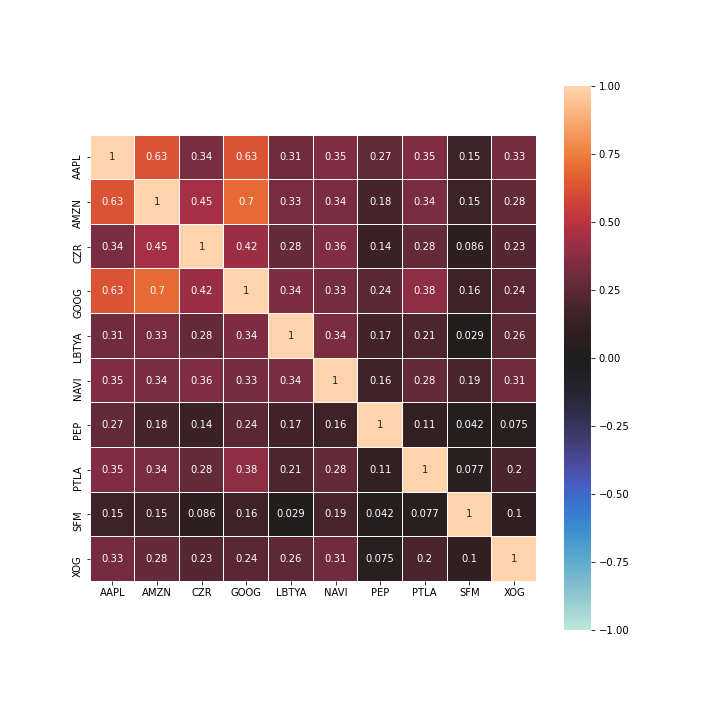
\includegraphics[scale=0.4]{corr}
\caption{Тепловая карты матрицы корреляций}
\label{fig:example_heatmap}
\end{figure}


Соответствующий матрице граф представлен на рисунке \ref{fig:example_graph}.

\begin{figure}[H]
\centering
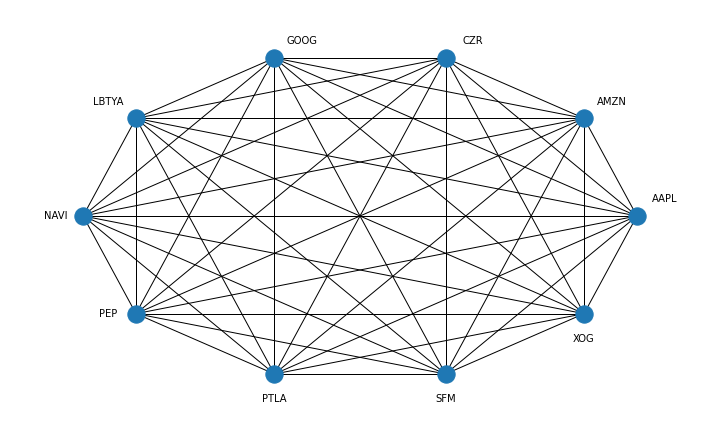
\includegraphics[scale=0.4]{graph}
\caption{Сетевая структура}
\label{fig:example_graph}
\end{figure}

Применим различные процедуры фильтрации.Из полученной сети построим максимальное остовное дерево.

\begin{figure}[H]
\centering
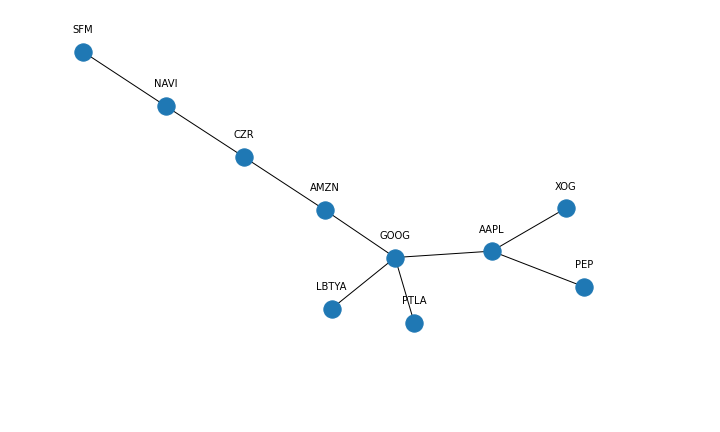
\includegraphics[scale=0.4]{mst}
\caption{Максимальное остовное дерево}
\label{fig:example_mst}
\end{figure}


Построим рыночный граф с порогом $\theta=0.3$. 


\begin{figure}[H]
\centering
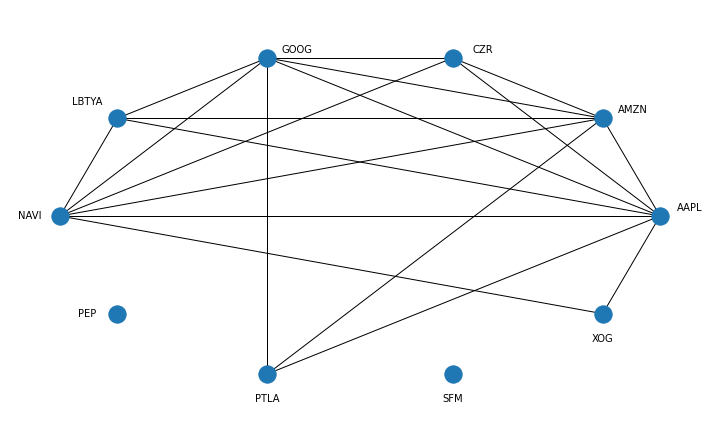
\includegraphics[scale=0.4]{mg}
\caption{Рыночный граф}
\label{fig:example_mst}
\end{figure}


В полученном рыночном графе найдём максимальную клику и максимальное независимое множество.

\begin{figure}[H]
\centering
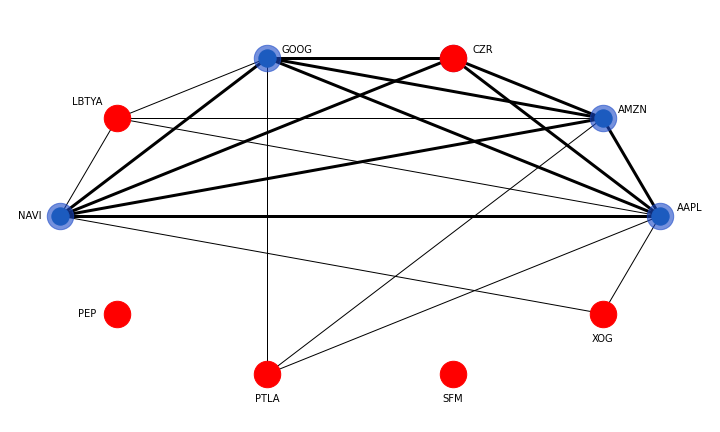
\includegraphics[scale=0.4]{mc_mis}
\caption{Максимальные клика и независимое множество}
\label{fig:mc_mis}
\end{figure}

Максимальная клика содержит 5 вершин, соединённых на рисунке \ref{fig:mc_mis} жирными линиями. Максимальное независимое множество содержит 6 вершин, одна из которых присутствует и в клике. Вершины, входящие в максимальное независимое множество отмечены на рисунке \ref{fig:mc_mis}  красным цветом.

